\documentclass[12pt]{article}
\usepackage{amsmath,amssymb,amsfonts,mathtools}
\usepackage[tagged, highstructure]{accessibility}
\usepackage[english]{babel}
\usepackage[utf8x]{inputenc}
\usepackage[T1]{fontenc}
\usepackage[margin=1in]{geometry}
\usepackage{scribe}
\usepackage{listings}
\usepackage{natbib,verbatim}

\usepackage{bbm}
\usepackage{hyperref}
\hypersetup{
    colorlinks=true,
    linkcolor=blue,
    filecolor=magenta,      
    urlcolor=magenta,
    citecolor=magenta,
    pdftitle={Midterm I},
    pdfauthor={Nisha Chandramoorthy},
    pdflang={en-US}
}

%\Scribe{Your Name}
\title{Midterm II}
\LectureNumber{CSE 6740}
\LectureDate{Due Nov 8th, '23 (6 pm ET)} 
\Lecturer{Total: 25 points}
\LectureTitle{Midterm II}

\lstset{style=mystyle}

\begin{document}
\MakeScribeTop

\section{Dimension reduction}
 Let our dataset $x_1,\cdots,x_m \in \mathbb{R}^d$ be arranged in the data matrix $X \in \mathbb{R}^{m \times d}$ with rows $X[i, :] = x_i^\top.$ Let the data be centered: $\sum_{i\in [m]} x_i = 0.$ Suppose $\mathrm{x}$ is a random variable chosen uniformly from the dataset.
\subsection*{Part I : 5 points}
Show that the first principal component is the $${\rm arg max}_{w\in \mathbb{R}^d:\|w\|=1} {\rm Var}(w^\top \mathrm{x}).$$
That is, the first principal component is the direction of maximum variance in the data.
\subsection*{Part II: 3 points}
Three students play a PCA-based game. The referee has access to (labeled) data in $d = 4$-dimensional space, but gives each student only 2 dimensions. In other words, each student has only two columns of $X,$ which are shown in Figure \ref{fig:pca}.
\begin{figure}[h]
    \centering
    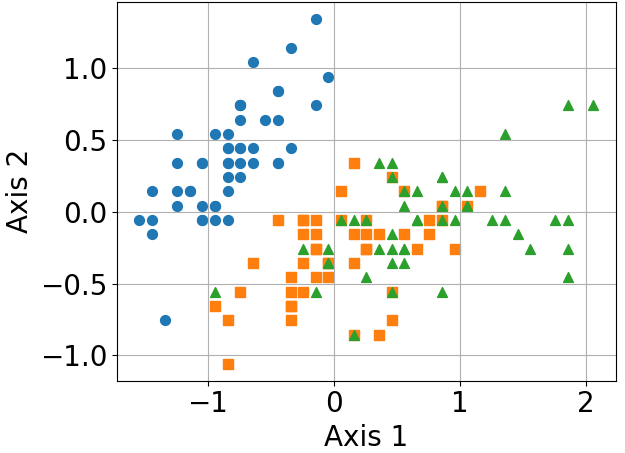
\includegraphics[width=0.3\textwidth]{midterm/pca-1.png}
    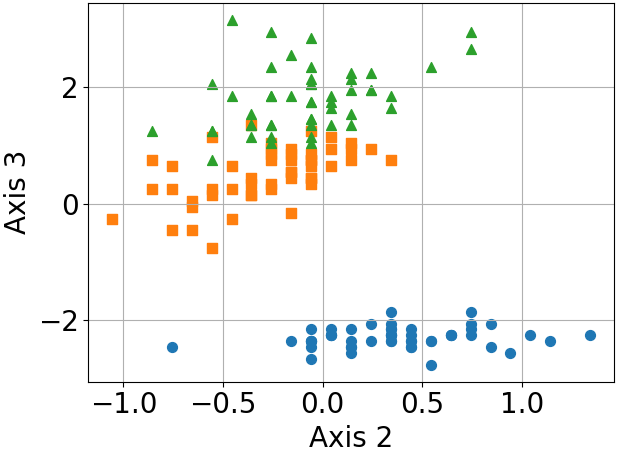
\includegraphics[width=0.3\textwidth]{midterm/pca-2.png}
    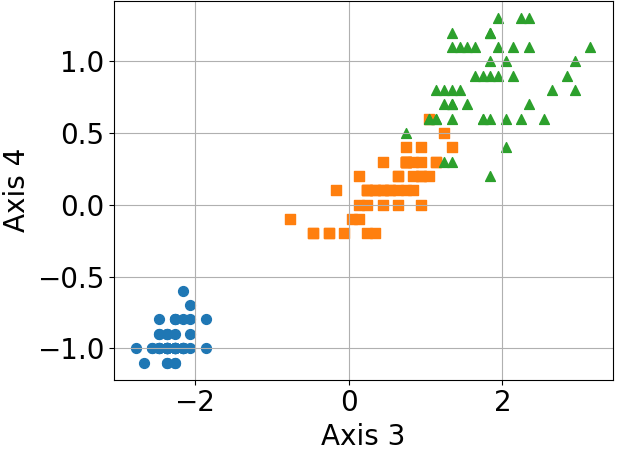
\includegraphics[width=0.3\textwidth]{midterm/pca-3.png}
    \caption{Data given to students 1 (left), 2 (center), and 3 (right) in Q1 part II.}
    \label{fig:pca}
\end{figure}
Suppose the first principal component (PC) of the original 4D data is $$v \approx [0.36138659, -0.08452251,  0.85667061,  0.3582892]^\top.$$ Each student, $i,$ ($i = 1, 2, 3$) calculates the first PC, $w_i,$ of the 2D data they are given. Identify whether each of the following statements is true or false and {\bf why}.    
    \begin{itemize}
        \item[(A)] In the set $\{w_1, w_2, w_3\},$ the vector $w_1$ is most aligned with $v.$ (2 points)
        \item[(B)] A principal component may not always be unique. (1 point)
    \end{itemize}
\subsection*{Part III: 2 points}
How can the students use the PCA of their data (Figure \ref{fig:pca}) to predict the labels (different colors/markers)? Give a heuristic algorithm (1 point). Which student will have the lowest training error if they followed your algorithm and why (1 point)?

\section{SVM and Kernel Trick}

\begin{figure}[h]
    \centering
    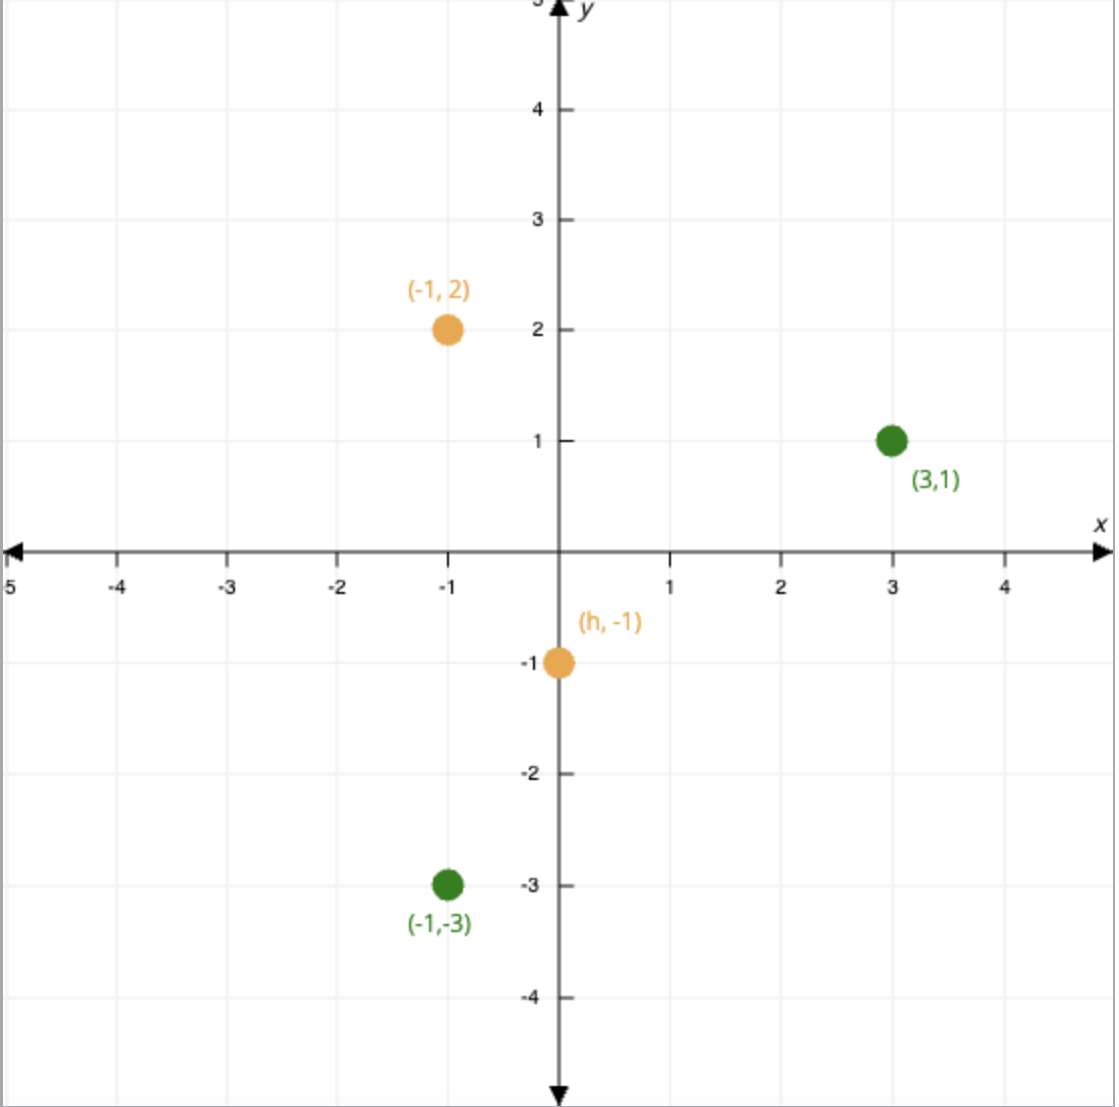
\includegraphics[width=0.5\textwidth]{midterm/SVM.png}
    \caption{Training Points}
    \label{fig:svm}
\end{figure}

Suppose we have four training examples, as Figure \ref{fig:svm}, in two dimensional space: positive examples at $x_1 = [-1,-3]^\top$ ,  $x_2 = [3,1]^\top$ ; negative examples at $x_3 = [-1,2]^\top$ ,  $x_4 = [h,-1]^\top$, where $h$ is a parameter such that $0\leq h \leq 3$. 
\subsection*{Part I (4 points)}
    What is the maximum value of $h$ such that the training points are still linearly separable? (4 points)
    \subsection*{Part II (2 points)}
    Derive a relationship between the margin achieved by a hard SVM classifier and $h$. (2 points)
    \subsection*{Part III (2 points)}
     Consider a polynomial kernel $K(\mathrm{x},\mathrm{y}) = (1 + \mathrm{x}\cdot \mathrm{y})^{p}$, $\mathrm{x},\mathrm{y}\in \mathbb{R}^2.$ Give a set of features $\phi(x)$ when $p = 2$ such that $k(\mathrm{x},\mathrm{y})=\phi(\mathrm{x})^\top \phi(\mathrm{y})$ (1 point). What is the dimension of the feature space? (1 point)
     \subsection*{Part IV (2 points)}
 Explain if true or false with an example. For any value of $h \geq 0,$ there is a kernel classifier $w^\top \phi(x)$ such that $w$ has only two non-zero entries. (2 points)
 

\section{Modified kernel ridge regression}
As usual, we have $m$ data points, $x_i \in \mathbb{R}^d, i \in [m],$ their corresponding outputs $y_i \in \mathbb{R},$ and a PD kernel $k$ on $\mathbb{R}^d\times \mathbb{R}^d.$ 
Consider the kernel regression problem,
\begin{align}
\label{eq:krr}
    {\rm arg min}_{\alpha \in \mathbb{R}^d} \alpha^\top K \alpha + (1/\lambda) \|K\alpha - Y\|^2,
\end{align}
where $K \in \mathbb{R}^{m\times m}$ is the Gram matrix with elements $K_{ij}= k(x_i, x_j)$ and $Y \in \mathbb{R}^m$ is the output vector with elements $y_i.$ In class, we learned that the solution of \eqref{eq:krr} gives the solution of the ridge regression problem in the RKHS corresponding to the kernel $k.$ That is, the ERM function in the RKHS is given by $h^*(x) = \sum_{i=1}^m \alpha_i k(x_i,x),$ where $\alpha \in \mathbb{R}^m$ is $\alpha = (K + \lambda I)^{-1} Y.$
\subsection*{Part I (1 point)}
Now suppose we have to make zero training error on some data points $(x_i, y_i),$ $i \in I \subseteq [m].$ Let the index set of these \emph{important} points be $I.$ Modify the problem \eqref{eq:krr} to incorporate this constraint. Specifically, add the constraints that for all $i \in I,$ $(K\alpha - Y)_i^2 = 0.$ (1 point).

\subsection*{Part II (2 points)}
Denote the dual variables you added in Part I as $c_i, i \in I.$
Show that the solution to the constrained optimization problem in Part I satisfies
$$\alpha = (I + D K)^{-1} D Y,$$ where $D$ is a diagonal matrix with entries $D_{ii} = 1/\lambda$ for $i \notin I$ and $D_{ii} = c_i,$ $i \in I.$ (2 points)

\subsection*{Part III (2 points)}
With your solution in Part II for $\alpha$ and $c,$ you try different cross-validation strategies to optimize for $\lambda$, the regularization parameter. 
Recall the $k$-fold cross validation algorithm. We select the regularization parameter that incurs the minimum CV loss. 
Match each strategy to an outcome on the right column and explain {\bf why}.
\begin{table}[h]
    \centering
    \begin{tabular}{p{0.35\linewidth} | p{0.6\linewidth}}
        Strategy & Outcome  \\
        \hline \\
         (A): $|I|$ iterations of CV, where we test on 1 important point at each iteration  & Not a valid strategy \\
         (B): $m - |I|$ iterations of CV, where we test on 1 unimportant point at each iteration.  & a valid strategy \\
         (C): $m$ iterations of CV or in other words, we calculate the leave-one-out error.  & only possible valid strategy\\
          & Best possible valid strategy \\
          \hline
    \end{tabular}
    \caption{Strategies and (scrambled) outcomes for Q3 Part III}
    \label{tab:my_label}
\end{table}


\end{document}
